% Signature figure — compile: pdflatex tsgg_signature.tex
\documentclass[border=4pt]{standalone}
\usepackage{tikz}
\usetikzlibrary{arrows.meta,positioning,fit,backgrounds,calc}

\begin{document}
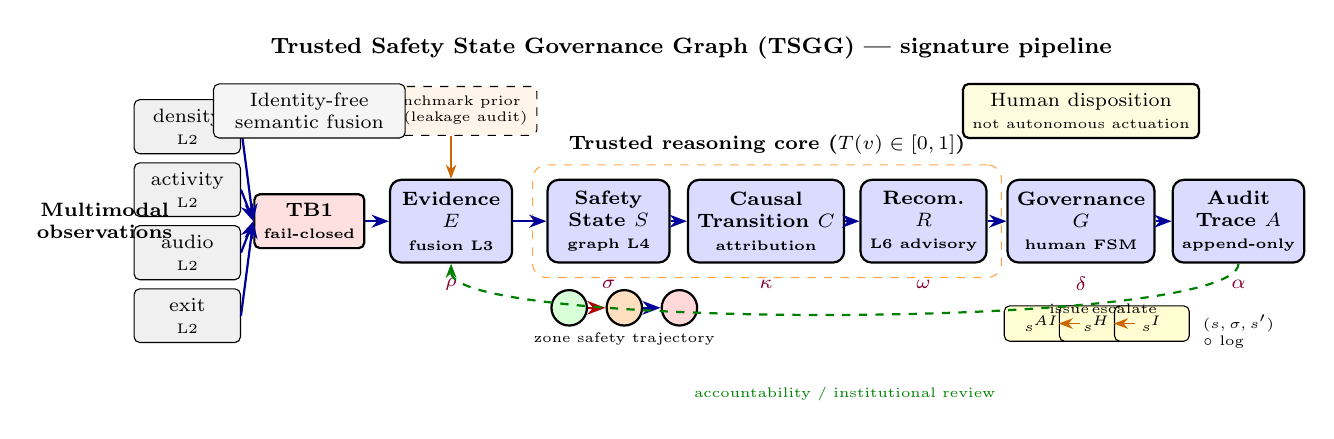
\begin{tikzpicture}[
  font=\sffamily,
  input/.style={draw, rounded corners=2pt, minimum height=0.55cm, minimum width=1.35cm,
                align=center, font=\scriptsize, fill=gray!12},
  gate/.style={draw, thick, rounded corners=2pt, minimum height=0.55cm, minimum width=1.1cm,
               align=center, font=\scriptsize\bfseries, fill=red!12},
  stage/.style={draw, thick, rounded corners=4pt, minimum width=1.55cm, minimum height=1.05cm,
                align=center, font=\scriptsize\bfseries, fill=blue!14},
  op/.style={font=\scriptsize\itshape, text=purple!70!black},
  flow/.style={-{Stealth[length=2.2mm]}, thick, draw=blue!60!black},
  trustflow/.style={-{Stealth[length=1.8mm]}, semithick, draw=orange!80!black},
  auditflow/.style={-{Stealth[length=1.8mm]}, dashed, thick, draw=green!50!black},
  fsm/.style={draw, rounded corners=2pt, minimum width=0.95cm, minimum height=0.45cm,
              align=center, font=\tiny\bfseries, fill=yellow!18},
  state/.style={circle, draw, thick, minimum size=4.5mm, inner sep=0pt, font=\tiny},
  labeltop/.style={font=\footnotesize\bfseries, text=black},
]

% --- Title band ---
\node[labeltop] at (6.4,3.35) {Trusted Safety State Governance Graph (TSGG) --- signature pipeline};

% --- Multimodal inputs (Information Fusion entry) ---
\node[input] (dens) at (0,2.35) {density\\{\tiny L2}};
\node[input] (act) at (0,1.55) {activity\\{\tiny L2}};
\node[input] (aud) at (0,0.75) {audio\\{\tiny L2}};
\node[input] (exit) at (0,-0.05) {exit\\{\tiny L2}};
\node[font=\scriptsize\bfseries, align=center] at (-1.05,1.15) {Multimodal\\observations};

\node[gate] (tb1) at (1.55,1.15) {TB1\\{\tiny fail-closed}};
\draw[flow] (dens.east) -- (tb1.west);
\draw[flow] (act.east) -- (tb1.west);
\draw[flow] (aud.east) -- (tb1.west);
\draw[flow] (exit.east) -- (tb1.west);

% --- Main pipeline stages ---
\node[stage] (ev) at (3.35,1.15) {Evidence\\$E$\\{\tiny fusion L3}};
\node[stage] (ss) at (5.35,1.15) {Safety\\State $S$\\{\tiny graph L4}};
\node[stage] (ct) at (7.35,1.15) {Causal\\Transition $C$\\{\tiny attribution}};
\node[stage] (rec) at (9.35,1.15) {Recom.\\$R$\\{\tiny L6 advisory}};
\node[stage] (gov) at (11.35,1.15) {Governance\\$G$\\{\tiny human FSM}};
\node[stage] (atr) at (13.35,1.15) {Audit\\Trace $A$\\{\tiny append-only}};

\draw[flow] (tb1) -- (ev);
\foreach \a/\b in {ev/ss, ss/ct, ct/rec, rec/gov, gov/atr} {
  \draw[flow] (\a) -- (\b);
}

% Operators under stages
\node[op] at (3.35,0.35) {$\rho$};
\node[op] at (5.35,0.35) {$\sigma$};
\node[op] at (7.35,0.35) {$\kappa$};
\node[op] at (9.35,0.35) {$\omega$};
\node[op] at (11.35,0.35) {$\delta$};
\node[op] at (13.35,0.35) {$\alpha$};

% Mini safety-state graph under S
\node[state, fill=green!15] (n1) at (4.85,0.05) {};
\node[state, fill=orange!25] (n2) at (5.55,0.05) {};
\node[state, fill=red!15] (n3) at (6.25,0.05) {};
\draw[thick, red!70!black, -{Stealth}] (n1) -- (n2);
\draw[thick, blue!60!black, -{Stealth}] (n2) -- (n3);
\node[font=\tiny] at (5.55,-0.35) {zone safety trajectory};

% Mini governance FSM under G
\node[fsm] (sai) at (10.85,-0.15) {$s^{AI}$};
\node[fsm] (sh) at (11.55,-0.15) {$s^{H}$};
\node[fsm] (si) at (12.25,-0.15) {$s^{I}$};
\draw[trustflow] (sai) -- node[above, font=\tiny] {issue} (sh);
\draw[trustflow] (sh) -- node[above, font=\tiny] {escalate} (si);

% Audit chain under A
\node[font=\tiny, align=left] at (13.35,-0.25) {$(s,\sigma,s')$\\$\circ$ log};

% Trust band
\begin{scope}[on background layer]
  \node[draw=orange!70, dashed, rounded corners=5pt, inner sep=5pt,
        fit=(ss)(ct)(rec), label={[font=\scriptsize\bfseries]above:Trusted reasoning core ($T(v)\in[0,1]$)}] {};
\end{scope}

% Benchmark prior
\node[draw, dashed, rounded corners=2pt, fill=orange!8, font=\tiny, align=center,
      minimum width=1.6cm] (prior) at (3.35,2.55) {Benchmark prior\\$\pi_0$ (leakage audit)};
\draw[trustflow] (prior.south) -- (ev.north);

% Human disposition callout
\node[draw, thick, rounded corners=2pt, fill=yellow!12, font=\scriptsize, align=center]
      at (11.35,2.55) {Human disposition\\{\tiny not autonomous actuation}};

% Accountability loop
\draw[auditflow] (atr.south) .. controls +(0,-0.85) and +(0,-0.85) .. (ev.south);
\node[font=\tiny, text=green!50!black] at (8.35,-1.05) {accountability / institutional review};

% Fusion contribution callout (IF lens)
\node[draw, rounded corners=2pt, fill=gray!8, font=\scriptsize, align=center,
      text width=2.2cm] at (1.55,2.55) {Identity-free\\semantic fusion};

\end{tikzpicture}
\end{document}
